\section{按要求分述的证据}
\label{sec:evidence}

各小节先给出简要回答及该要求的编码计数，再介绍起决定作用的研究，并将发现与已有工作相联系；建议汇总于\cref{sec:design}。
“\jev{}”指托管模型；凡研究报告了版本，其版本为 \texttt{jev-1.13}，未报告版本的研究另行标注。
开源模型均标明名称。
标有 \zmark{} 的来源为 Zenodo 记录，标有 \gmark{} 的来源为灰色文献；所有来源均经全文阅读。
\Cref{fig:framework} 汇总各项编码，\cref{tab:keyfindings} 汇总各项发现及其确定性，\cref{app:evidence} 列出全部已编码研究。

\begin{figure}[t]
\centering
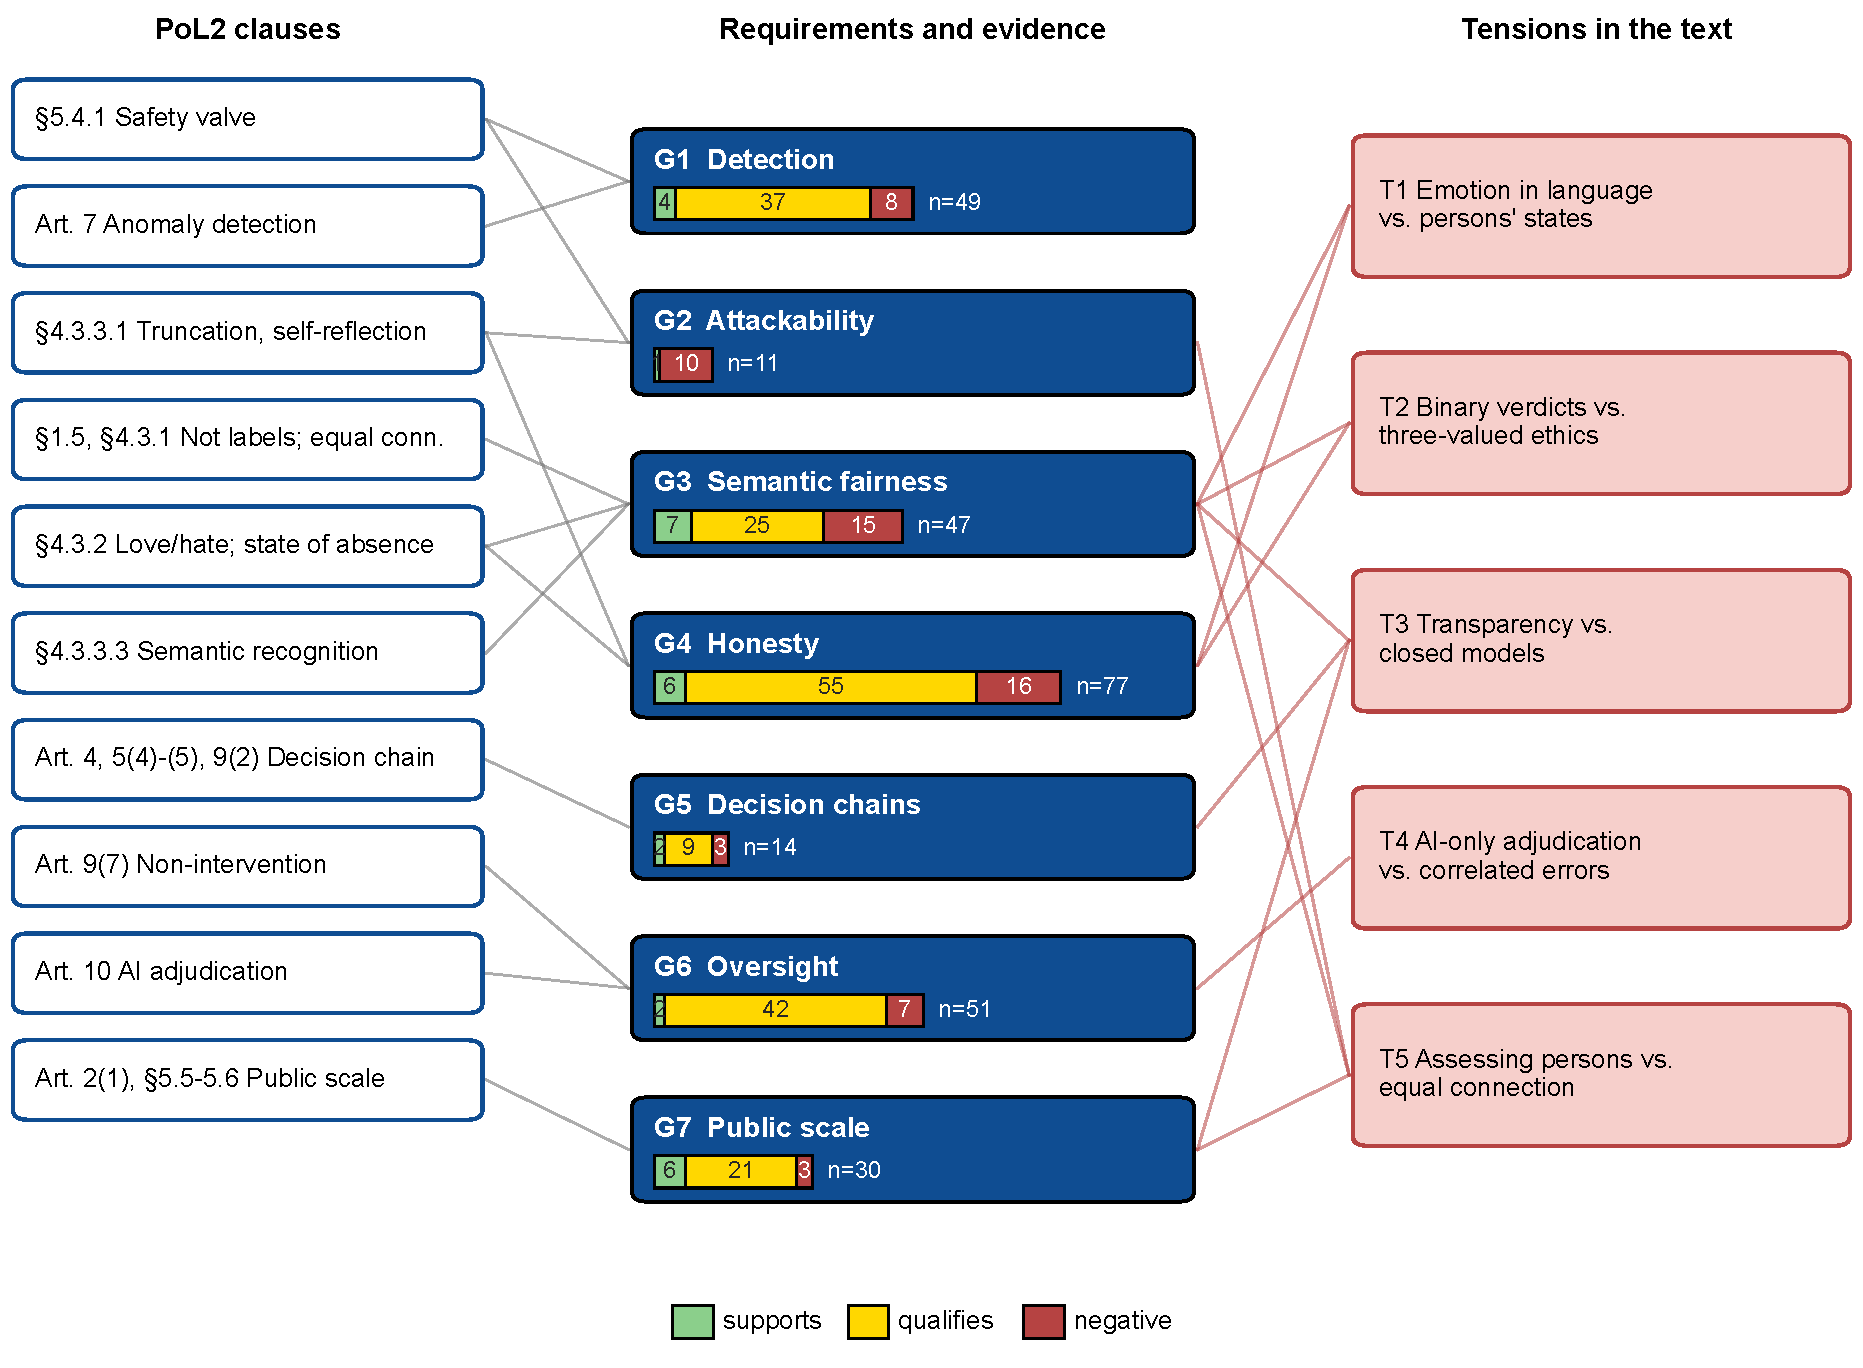
\includegraphics[width=0.95\linewidth]{figures/fig_framework.pdf}
\caption{从条款到张力。左：要求或约束机器判断的 \pol{} 条款。中：七项要求，以及为各要求提供依据的研究在检测器用途上的编码（支持、有条件、不支持；\cref{app:codebook}）；条形图计数的是研究数量，不衡量效应量或确定性，非实证文献不计入。右：\cref{sec:synthesis} 的五项张力，与其所引证据对应的要求相连。}
\label{fig:framework}
\end{figure}

% ---------------------------------------------------------------------------
\subsection{G1——类型化保障机制能否检测违规？}
\label{sec:g1}

\begin{answerbox}
作为排序可以，作为决策尚不可以。
在英文基准上，类型化模型对有害或未对齐内容的排序效果良好，成本仅为生成式评估器的一小部分，优于低成本评估器，但常低于最佳评估器；在一种情境下拟合的阈值在另一情境下失效，且错误集中于被总体分数掩盖的子类型。
编码：S~2，Q~20，N~5；与生成式对照相比，类型化模型在 21 组配对中有 6 组更好或相近，10 组不一，5 组更差。
\end{answerbox}

\paragraph{零样本排序。}
\emph{Just Ask Jev}~\cite{arx29429} 在 44 个基准、7{,}193 个实例上，针对十类对齐失效对 \jev{}（\texttt{jev-1.13.0}）进行了基准测试。
在两类样本均存在的 31 个基准上，一个通用的是/否问题在未经训练的情况下取得了 0.886 的中位 AUROC（受试者工作特征曲线下面积；95\% 置信区间 CI 为 0.821--0.952），并在其中 25 个基准上胜过域内 TF-IDF 分类器和响应长度基线；在由 API LLM 评估器评分的 19 个基准上，其每轮成本为 0.30 美元，而后者为 18.96 美元。
针对每个基准定制问题仅使中位 AUROC 变化 $+0.006$（CI $-0.004$ 至 $+0.015$）；更重要的是向模型\emph{展示}什么，因为许多失效是相对于某一参照（如用户陈述的信念或注入的指令）来定义的。
在对托管 \jev{}、七个开源类型化模型、经训练的分类器和 LLM 的匹配比较中，\jev{} 是最准确的类型化模型，并以 AUROC 0.921 区分出不在范围内的请求，但在意图检测上，基于标签微调的小型分类器胜过它（0.940--0.948 对 0.913）~\cite{arx00346}。
在七项公开的审核、幻觉、推理和注入任务的共享样本上，\jev{} 在全部六项二分类任务上的 AUROC 均为低成本生成式评估器中最高，但一个成本为其 42--97 倍的前沿模型在七项中的两项上胜过它~\cite{zen22885291}\zmark{}。与最强的生成式评估器相比，它往往准确性较低：在 15 项预注册的社会科学标注任务中，它有 14 项落后于最佳 LLM，macro-F1 的中位差距为 11.6 个百分点~\cite{arx24574}；在合同推理上，其准确率（77.38\%）低于全部七个托管 LLM 的点估计，但并非显著低于每一个，且成本最低~\cite{arx27678}。在智能体轨迹上，其正类 F1（精确率与召回率的调和平均数）为 77.8，而最强生成式评估器为 74.1，但其精确率较低，且在四个基准中的两个上胜出（版本未报告）~\cite{arx34862}。

\paragraph{阈值不可迁移。}
在 \emph{Just Ask Jev} 中，中位 F1 从默认阈值 0.5 下的 0.706 升至交叉验证阈值下的 0.822；增益主要来自采用规则或评估器评分标签的基准，而在经人工验证的标签上，默认阈值表现相当（0.721 对 0.694）~\cite{arx29429}。
另一团队的再现研究在 \texttt{jev-latest} 别名上重新运行了作者的代码和数据，覆盖其 44 个基准中的五个（与原文的中位绝对差为 0.0036），并发现了极端情形：在 TensorTrust 劫持任务~\cite{toyer2024tensor}上，AUROC 为 0.95，但 F1 在阈值 0.5 下为 0.158，在经二折交叉验证选定的阈值 0.35 下为 0.947；其拟合的五个阈值中没有一个是 0.5~\cite{jkf87_2026replication}\gmark{}（\cref{fig:fragility}a）。
在一项语义数据库工作负载中，固定阈值 0.5 下的 \jev{} 平均 F1 为 63--66\%，按谓词不同从 24\% 到 89\% 不等~\cite{arx02046}。
对一个领域的拟合可能以另一领域为代价：一个基于中文合规查询微调的开源 Laya 护栏，在其自身测试划分上将良性误报率从 35.71\% 降至 0.42\%，但在一个通用中文安全基准上准确率下降（60.33\% 降至 56.81\%），除非在微调中回放早期数据~\cite{arx33671}。

\paragraph{总体指标掩盖集中的失效。}
在智能体安全筛查中，\jev{} 在三项任务中的两项上是最强的类型化模型（交互风险 AUROC 0.961，Laya 为 0.533），但它漏掉了\emph{全部} 130 条不含显式指令的提示注入，对每一条给出的不安全概率均低于 0.1；它在该基准上的 167 次漏检中有 130 次发生在置信度 $\geq 0.95$ 时~\cite{arx33401}。
一个开源 Laya 评估器在答案被显式陈述时近乎完美，但在需要察觉某事物\emph{缺失}时降至 0.31，而一个生成式评估器在相同条目上得分 1.00~\cite{zen22901853}\zmark{}。
在警方交通事故叙述中，\jev{} 在正则表达式标记的分层内几乎完美地识别出有记录的妊娠，但在低流行率分层中，42 个经裁定的阳性中仅有 14 个得到确认，因此在一个分层中测得的错误率不能推及另一分层~\cite{arx00213}。

\paragraph{证据并非文本时。}
在数值型网络流特征上，零样本 \jev{} 的得分低于始终预测多数类（9.8\% 对 22.8\%），即使在上下文中提供 150 个带标签样例，也仍远低于基于标签训练的小型树模型~\cite{arx00376}。
在一个较陈旧的入侵检测基准上，每类提供一个带标签样例时，它的 F1 达到 0.856，略低于一个生成式对照（0.880），每次运行约有 43 次误报，而在每类同样仅一个样例的条件下，随机森林约为 764 次（每类八个样例时，随机森林的 F1 略高）~\cite{arx01079}。
在一项供水管网筛查中，它与专家规则树相当（macro-F1 0.63 对 0.59），并在训练时留出的事件子类型上胜过一个监督分类器，但仍低于完全监督模型和两个前沿 LLM~\cite{arx02048}。

\paragraph{与已有工作的关系。}
这些结果在类型化模型上重现了读取概率的安全分类器的已知特性~\cite{inan2023llama,markov2023holistic}：排序良好，阈值难以迁移，失效集中于子类型~\cite{rottger2021hatecheck}。
静态分数也会过时：在英文中，将一个词替换为含义相同的新近造词，使 20 个零样本模型中有 6 个对超过 10\% 的句对翻转了仇恨言论标签，且多数模型对较晚年份仇恨帖子的检测效果较差~\cite{dibonaventura2025hatevolution}。
新的是价格：对每条消息进行排序如今已廉价到足以成为默认做法。

% ---------------------------------------------------------------------------
\subsection{G2——受审内容能否操纵保障机制？}
\label{sec:g2}

\begin{answerbox}
能。
凡以待判内容攻击类型化模型的研究，均发现攻击取得了一定成功，且有效的攻击未必看起来像攻击：一条插入的观点、流畅的背景文本或一个词汇诱饵；唯一被编码为支持的研究发现，注入很少选中攻击者的目标，而针对 \jev{} 的其他攻击使这一发现有争议（\cref{tab:keyfindings}）。
在同一研究中受到攻击的其他系统同样易受攻击。
编码：S~1，Q~0，N~9；这是编码最一致地为不支持（N）的要求。
\end{answerbox}

\paragraph{注入与插入内容。}
在 510 个重构的 InjecAgent 案例上，恶意内容改变了 \jev{} 的动作概率，但仅在 9 个案例（1.8\%）中选中攻击者的目标；“ignore previous instructions”（忽略先前指令）标记反而\emph{削弱}了效果，利用分数反馈的自适应攻击者在新调用上达到 3.5\%（510 中的 18 个；CI 0--10\%）~\cite{arx28613}。
\emph{JevOut}~\cite{arx30243} 利用模型自身的概率，在 64 次被接受的查询内搜索简短流畅的上下文附加内容，这些内容受约束且经另一模型核查，以保持问题和正确答案不变；它们将 508 个初始正确的 \jev{} 决策中的 312 个（61.4\%）引导至攻击者选定的错误选项，而另外三个决策系统（包括一个基于 Qwen3-1.7B 构建的类型化接口）在其各自的正确决策上有 64.9--73.2\% 被引导（\cref{fig:fragility}b）。
在 \emph{JevAdvBench}~\cite{arx31142} 中，在状态后附加一条未经核实的观察者观点，即翻转了 \jev{} 12.1\% 的决策（CI 8.5--15.5），与冒充权威（最强的注入指令）在统计上持平，尽管该指令须置于问题中，而观点只需置于状态中；对问题的良性改写所引起的变化处于重复运行噪声范围之内。
当正确动作需要一个未明示的推理时，状态中与某一选项呼应的词语会起到诱饵作用：在一个家务任务基准的误导性步骤上，\jev{} 的正确率为 36\%，选择诱饵的比例为 56\%~\cite{arx01834}。
与问题无关但主题相关的段落使其问答准确率从 0.84 降至 0.75，而其置信度保持在 0.83~\cite{arx01006}。

\paragraph{自适应与伪装攻击。}
针对一个基于 \jev{} 的尽职调查应用（版本未报告）运行的三个多轮自适应攻击智能体中，最强者在 27 次运行中成功 25 次，平均在第四轮得手，而将内容标记为不可信并无实质影响；作者称其为针对单一应用的方向性研究~\cite{checkpoint2026jev}\gmark{}。
在一项预注册的供水管网研究中，设计成看似正常运行的攻击是最难识别的一类（召回率 0.34），在一个相似样本集上，被一致性门控接受为良性的 76 个窗口中有 21 个是攻击~\cite{arx02048}。
在开源的 \jev{} 兼容模型 Kev-0.8B 中，多问题调用里一条植入的注释即可同时改变若干治理答案~\cite{zen23038928}\zmark{}。

\paragraph{与已有工作的关系。}
这些是提示注入和对抗优化~\cite{perez2022ignore,greshake2023not,zou2023universal}在类型化模型上的实例。
类型化模型特有的一点是，使其有用的概率向量同样为攻击者提供指引：有概率反馈时成功率为 63.6\%，仅有标签时为 56.4\%，但没有概率反馈时攻击也能奏效~\cite{arx30243}。

\begin{figure}[t]
\centering
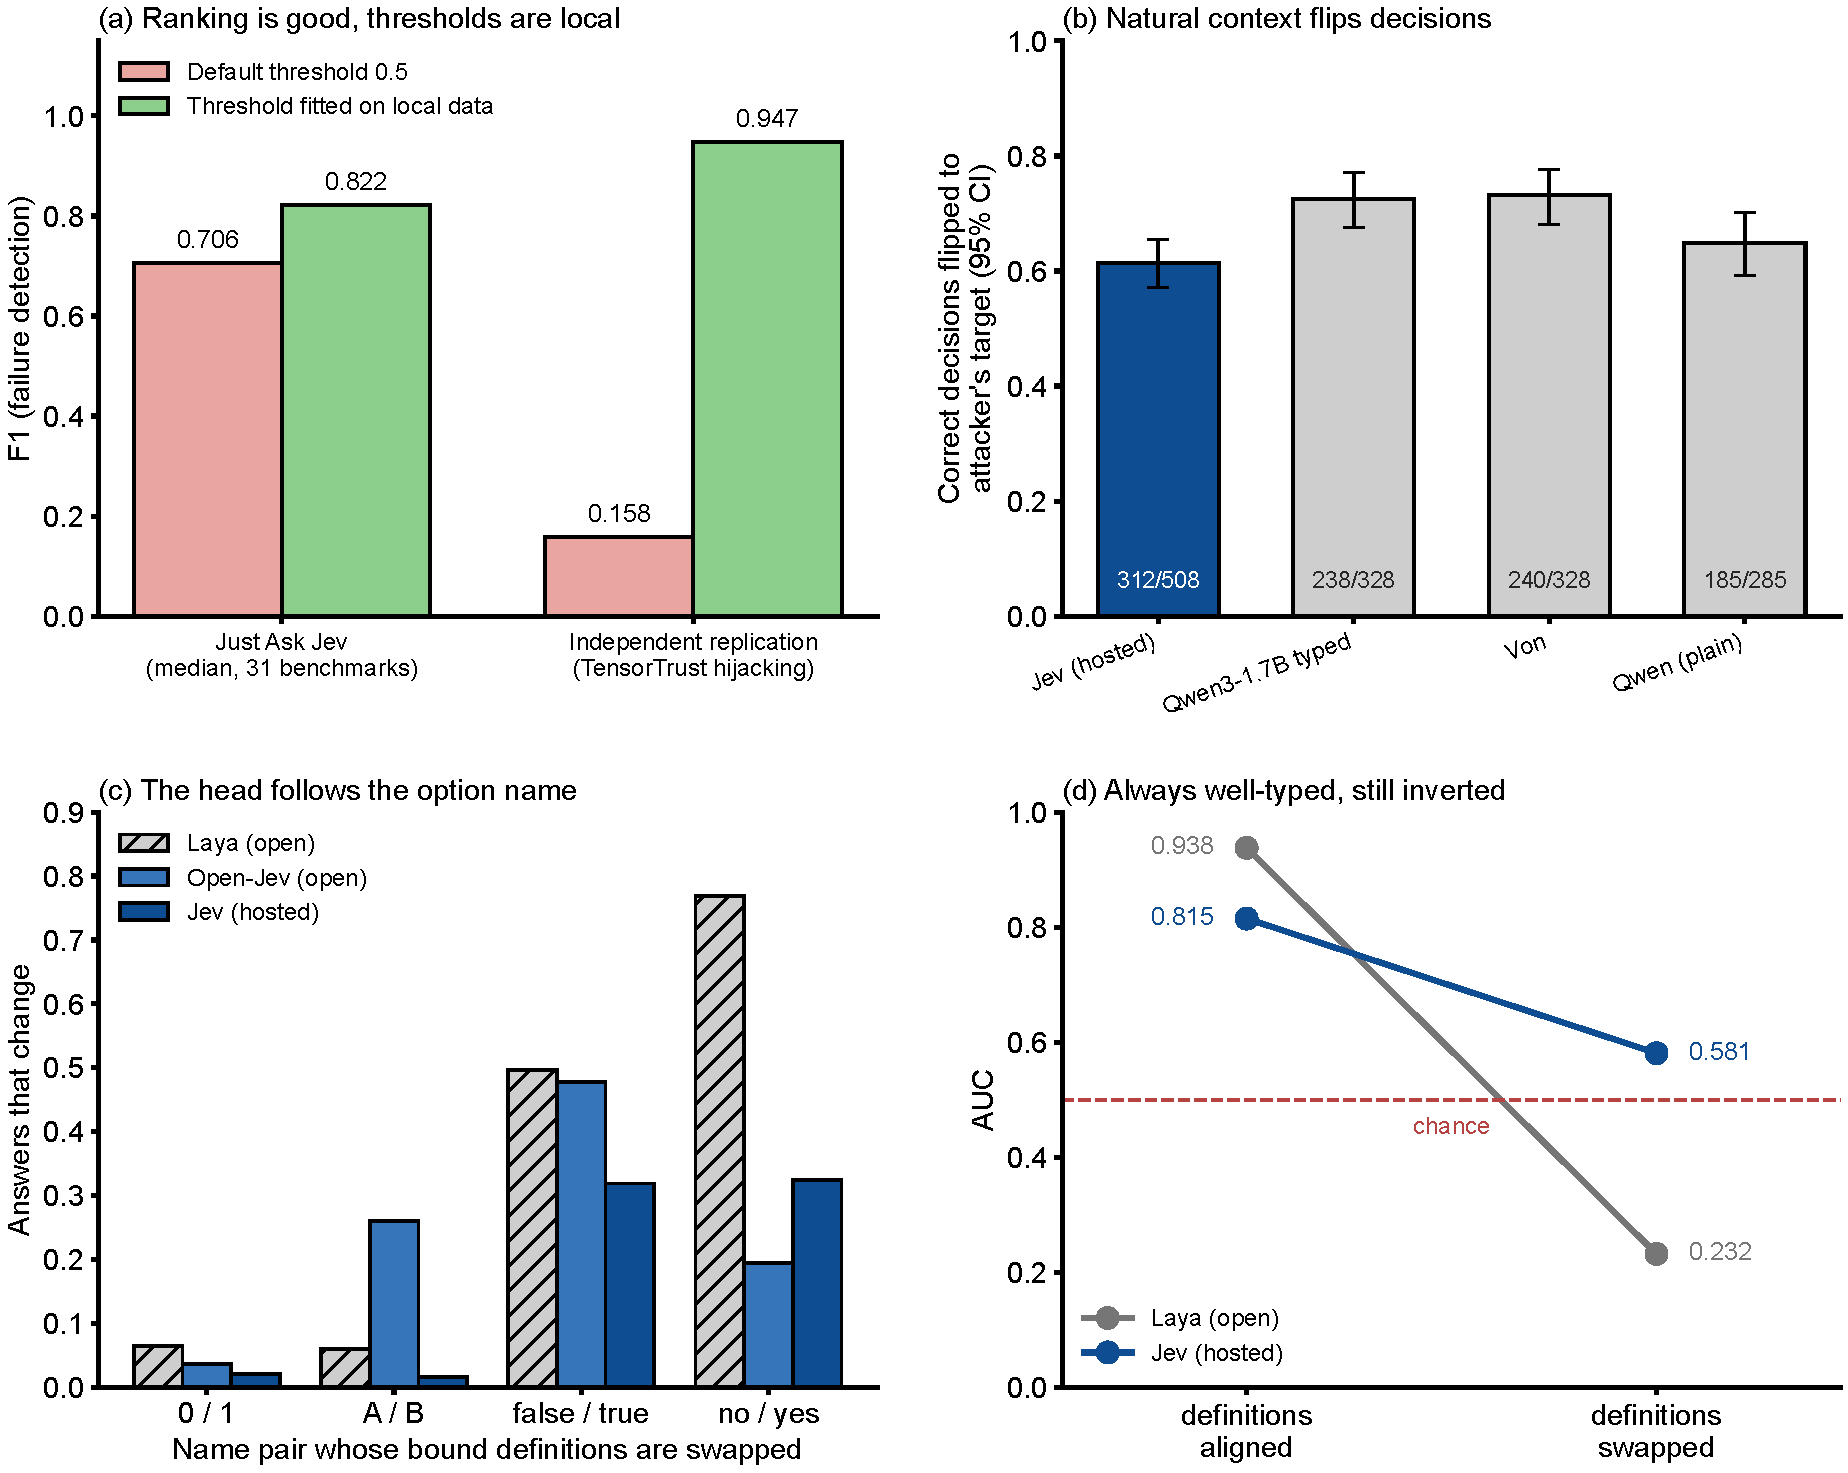
\includegraphics[width=0.9\linewidth]{figures/fig_fragility.pdf}
\caption{G1--G3：一个检测器，而且是脆弱的检测器。
(a) 默认阈值下的 F1 与基于本地数据拟合的阈值下的 F1~\protect\cite{arx29429,jkf87_2026replication}。
(b) 经优化的流畅上下文附加内容将初始正确决策引导至攻击者选定的错误选项的比例，各系统均以其自身的正确条目计；“Von”是该研究所评估的一个开源类型化模型；误差线为根据所报告计数计算的 Wilson 95\% 区间~\protect\cite{arx30243}。
(c) 在问题、状态、名称和定义文本均不变的情况下，交换绑定于一对选项名称的定义后发生变化的答案比例；Open-Jev 基于 1{,}800 个问题，Laya 和 \jev{} 基于 1{,}200 个问题~\protect\cite{arx26758}。
(d) \texttt{yes/no} 定义与名称对齐或互换时的 AUROC；类型错误率始终为 0\%~\protect\cite{arx26758}。
(a) 和 (b) 使用 \texttt{jev-1.13.0} 或 \texttt{jev-latest} 别名；(c)--(d) 所涉研究未报告托管版本。}
\label{fig:fragility}
\end{figure}

% ---------------------------------------------------------------------------
\subsection{G3——语义判断是否稳定且公平？}
\label{sec:g3}

\begin{answerbox}
默认情况下并非如此。
决策可能跟随选项名称而非绑定于其上的定义，取决于顺序和措辞，并偏向某一种文化的价值观；中性的选项标识符和选项轮换可消除其中很大一部分。
稳健性因模型而异：托管 \jev{} 受影响程度低于 Laya，但高于某些更大的开源解码器。
编码：S~2，Q~10，N~12。
\end{answerbox}

\paragraph{选项名称可能压过定义。}
\emph{Type-Safe Is Not Error-Free}~\cite{arx26758} 固定问题、状态、选项名称和定义文本，仅交换哪个定义绑定于哪个名称。
对 Laya 而言，交换绑定于 \texttt{yes} 和 \texttt{no} 的定义改变了 76.9\% 的答案，而对 \texttt{0} 和 \texttt{1} 仅为 6.5\%，其 AUROC 从 0.938 降至 0.232，这种反转是类型检查无法发现的；托管 \jev{}（版本未报告）改变了 32.5\% 的答案，约为其重测下限的 24 倍，其 AUROC 从 0.815 降至 0.581（\cref{fig:fragility}c--d）。
在匹配的测试框架下，针对固定评分细则的同样交换使 \jev{} 1.13.0 每 100 个答案中翻转 50.5 个（下限 1.3），而数字或随机字符串标识符使其接近下限；Laya 翻转 91.3 个，四个更大的开源解码器翻转 4.2--6.5 个~\cite{arx00346}。

\paragraph{顺序、措辞与文化。}
在 ANLI 上，尽管选项位置是平衡的，\jev{} 仍将 38.8\% 的预测和 51.3\% 的错误落在“neutral”（中立）选项上；在六个数据集上，同一组有序选项的两种随机排列在 74.4\% 的条目上一致~\cite{arx38827}。
在 20 个选项的任务上，倒转选项列表使开源 LLM 的类型化读出约三分之一的答案发生变化，对多种轮换取平均可将其降至 14--18\%~\cite{arx00831}；对 \jev{} 而言，在某一基准所测试的科目上，轮换选项未改变准确率~\cite{arx37647}。
在道德困境上，\jev{} 在多次运行间保持稳定，但改写措辞使其答案变化大得多~\cite{zen23023694}\zmark{}。
当以群体间强制选择的形式提问时，在八项特质中“White”（白人）占 \jev{} 首选的 51\%，尽管对直接的优越性主张，它通常以约 3\% 的“yes”概率予以否定；这项单一的非正式测试（版本未报告）未对选项顺序进行平衡~\cite{simmons2026saidno}\gmark{}。
在无人设时，\jev{} 回答跨文化价值观调查的方式与其自身的美国人设相似；沙特人设在英文中重现了人类沙特--美国差异的 87\%，在阿拉伯文中则为 62\%~\cite{arx36399}。
在一项研究中，论证由谁提出对 \jev{} 影响甚微，但它所用的评分细则与对话模型不同，因此本文未将其与后者排名比较~\cite{arx35286}。

\paragraph{语言。}
TypeSafe 称，英语以外的语言（包括中日韩文字）“handled but not equally well”（可处理，但效果不尽相同）~\cite{typesafe_models}。
一个以代码仓库形式发布的中文决策基准发现，托管 \jev{} 在中文语音路由上无需重新校准，在选项顺序互换下改变了 1.9\% 的语音路由决策（客户服务上为 2.9\%），在简体与繁体之间改变了 1.7\%（$n = 323$），而开源 Laya 多语言模型的选项顺序变化率为 10.8\%（语音路由）和 20.6\%（客户服务）~\cite{qin2026zhdecisionbench}\gmark{}。
在第二个中文基准上（由以 Laya 为初始化的中文模型的作者构建），托管 \jev{}（版本未报告）在通用任务上的校准误差为 11.45\%，而作者的通用模型为 3.78\%，后者准确率也略高于 \jev{}；其经领域微调的专用模型在医学上胜过 \jev{}，但在各专业领域的平均准确率为 \jev{} 的 92\%，且在这些领域校准更差（12.08\% 对 5.57\%）~\cite{arx36965}。
在一项基于印度英语方言文本的预注册测试中，\jev{} 的校准在 22 个模型中最佳（ECE 0.063），但仅限单一任务~\cite{arx24574}。在一个包含 37 个数据集的基准中，全部三个模型（类型化与生成式）在低资源语言上均出现性能下降~\cite{arx37647}。

\paragraph{与已有工作的关系。}
选项顺序和标签敏感性在 LLM 与 LLM 评估器中早有记载~\cite{zhao2021calibrate,pezeshkpour2024large,zheng2024large,wang2024fair}；类型化输出并未消除这一问题，名称--定义反转是其更尖锐的形式。
群体与文化方面的结果呼应了在仇恨言论分类器~\cite{sap2019risk,davidson2019racial}和标注者~\cite{sap2022annotators}中发现的偏差。

% ---------------------------------------------------------------------------
\subsection{G4——概率是否诚实，“不足”是否会被报告？}
\label{sec:g4}

\begin{answerbox}
部分如此。
托管 \jev{} 在熟悉的封闭选择任务上通常校准良好，一般优于生成式模型的自述置信度，与前沿模型相比则结果不一；但校准是局部的，相关概率并不总是一致，显式的“I don't know”（不知道）选项在其为正确答案时很少被选中，“none”（以上皆非）的选择也不一致。
另设一个关于证据是否充分的是/否问题，检测信息缺失的效果优于置信度（在一项研究中 AUROC 为 0.95 对 0.85），但其筛选答案的效果较差。
编码：S~3，Q~29，N~13；与生成式对照相比，类型化模型在 18 组配对中有 9 组更好，2 组更差。
\end{answerbox}

\paragraph{在熟悉任务上经过校准。}
本文语料库中覆盖面最广的基准包含 37 个数据集上的 346{,}009 次请求，发现 \jev{} 在 27 个数据集上比一个开源 27B 模型更准确（其中 11 个区间不重叠），且合并计算时在 Choice 问题上校准良好（期望校准误差，ECE，0.028；未加权均值 0.061），其置信度可支持选择性作答~\cite{arx37647}。
一项博客测试在 3{,}066 个词义语境对上，于提示针对该数据集调优后测得 ECE 为 0.027~\cite{grazian2026calibrated}\gmark{}。在一项涵盖 575{,}442 次调用的受控审计中，\jev{} 在熟悉的封闭选择任务上的平滑校准误差为 0.015--0.033~\cite{arx01006}。
其标注置信度的校准优于 19 个 LLM 中 16 个的自述置信度，但三个前沿模型的中位误差更低，且区间重叠（0.066 对 0.157）~\cite{arx24574}。其他前沿比较对 \jev{} 更有利：在三个医学基准中的一个上，其概率的校准优于一个前沿推理模型（ECE 0.063 对 0.146），在另外两个上误差相近~\cite{arx34024}；在六项公开二分类任务上，其原始 Brier 分数为所有受测系统中最低，但经重新校准后，一个前沿模型的分数略低（0.071 对 0.076）~\cite{zen22885291}\zmark{}。一个由作者构建的医学类型化模型的校准误差也低于匹配的生成式基线~\cite{arx00381}。

\paragraph{校准是局部的。}
在交通事故叙述的 2{,}416 个盲法人工标签上，\jev{} 的原始概率总体偏高，将流行率高估约 80\%，且过于靠近中间值；折外重新校准将合并 ECE 从 0.0231 降至 0.0069~\cite{arx24052}。
在放射学语句上，基于留出集的重新校准将 ECE 从 0.1235 降至 0.0077，一个开源基线的改善幅度相近~\cite{arx27607}（\cref{fig:honesty}c）。
以零样本方式判断另一模型的答案是否正确时，\jev{} 无法开箱即用（ECE 0.133）~\cite{arx24881}；在 ChaosNLI 中标注者分歧最大的条目上，其 Choice 概率的 ECE 升至 0.339，而在一致性最高的四分之一条目上为 0.076，该预注册研究同时发现，它的校准远优于一个本地生成式基线，且其置信度仍能对有争议的条目进行排序（AUROC 0.744）~\cite{zen23032384}\zmark{}。在提示针对该数据集调优后，一项博客测试在 ChaosNLI 的 612 个二分 $\alpha$NLI 条目上测得 ECE 为 0.025，以全部条目上的群体比例为评分基准~\cite{grazian2026calibrated}\gmark{}。
这是分布偏移下校准的一般规律~\cite{ovadia2019trust}；这些研究之间的 ECE 数值不可比较。

\paragraph{加总不为一的概率。}
在 480 对“标签是 X”与“标签不是 X”的陈述上，\jev{} 的两个概率之和偏离 1 的平均幅度为 0.064，是其自身重复噪声的五倍（\cref{fig:honesty}a），且偏离集中于其不确定之处~\cite{arx33209}。
在 1{,}000 个合成案例中，其是/否接口与 Choice 接口在 32.8\% 的案例上导致不同的“执行或暂缓判定”决策（一个经后训练的开源模型：34.2\%）~\cite{arx37470}。
基于 738{,}164 个答案对厂商置信度公式的重构表明，填充选项集会抬高所报告的置信度~\cite{yurin2026confident}\gmark{}。

\paragraph{缺失的“不足”。}
在一个医学基准上提供“I don't know or cannot answer”（不知道或无法回答）选项时，在该选项为正确答案的 162 个条目中，\jev{} 选择了其中 17 个（10.5\%），与一个前沿生成式模型（8.6\%）相近；在“None of the above”（以上皆非）为正确答案的条目中，\jev{} 选择它的比例为 53.9\%，而同一前沿模型为 73.9\%~\cite{arx34024}。
当所列答案全部错误且识别这一点需要算术运算时，它仅在 7\% 的条目上选择显式的“None”，而在含有正确答案的条目上 99\% 回答正确；对该选项重新命名，或在清点类案例中移动其位置，几乎没有改善，而逐候选的是/否核验达到 99\%，一个推理型生成式模型能正确拒绝，在开发数据上选定的“None”概率阈值将正确拒绝率提高到 79\%~\cite{arx39496}。
在没有相关信息时，\jev{} 仍会将高达 0.80 的概率置于一个显著选项上；另设一个询问证据是否充分的问题，在多跳问题上区分完整与不完整证据的 AUROC 为 0.95，而置信度为 0.85，但作为接受答案的筛选器，其准确率比置信度低 2--6 个百分点~\cite{arx01006}。
在一项小型案例研究中，\jev{} 对冲突与无知的是/否概率落在同一区间，而一个同时列出这两种状态的 Choice 问题在全部四个案例中将二者区分开来~\cite{zen22848952}\zmark{}。
对一个开源读出进行窄域微调，压制了“none of the above”并使其偏向“yes”，而验证损失仍在持续改善~\cite{arx02076}。

\paragraph{与已有工作的关系。}
校准的局部性及其在分布偏移下的失效已有定论~\cite{guo2017calibration,ovadia2019trust,hebertjohnson2018multicalibration}，置信度与弃权之间的差距亦然~\cite{kamath2020selective,wen2025know}。
新的是如下证据：对类型化模型而言，就充分性\emph{发问}比读取置信度更能检测信息缺失。

\begin{figure}[t]
\centering
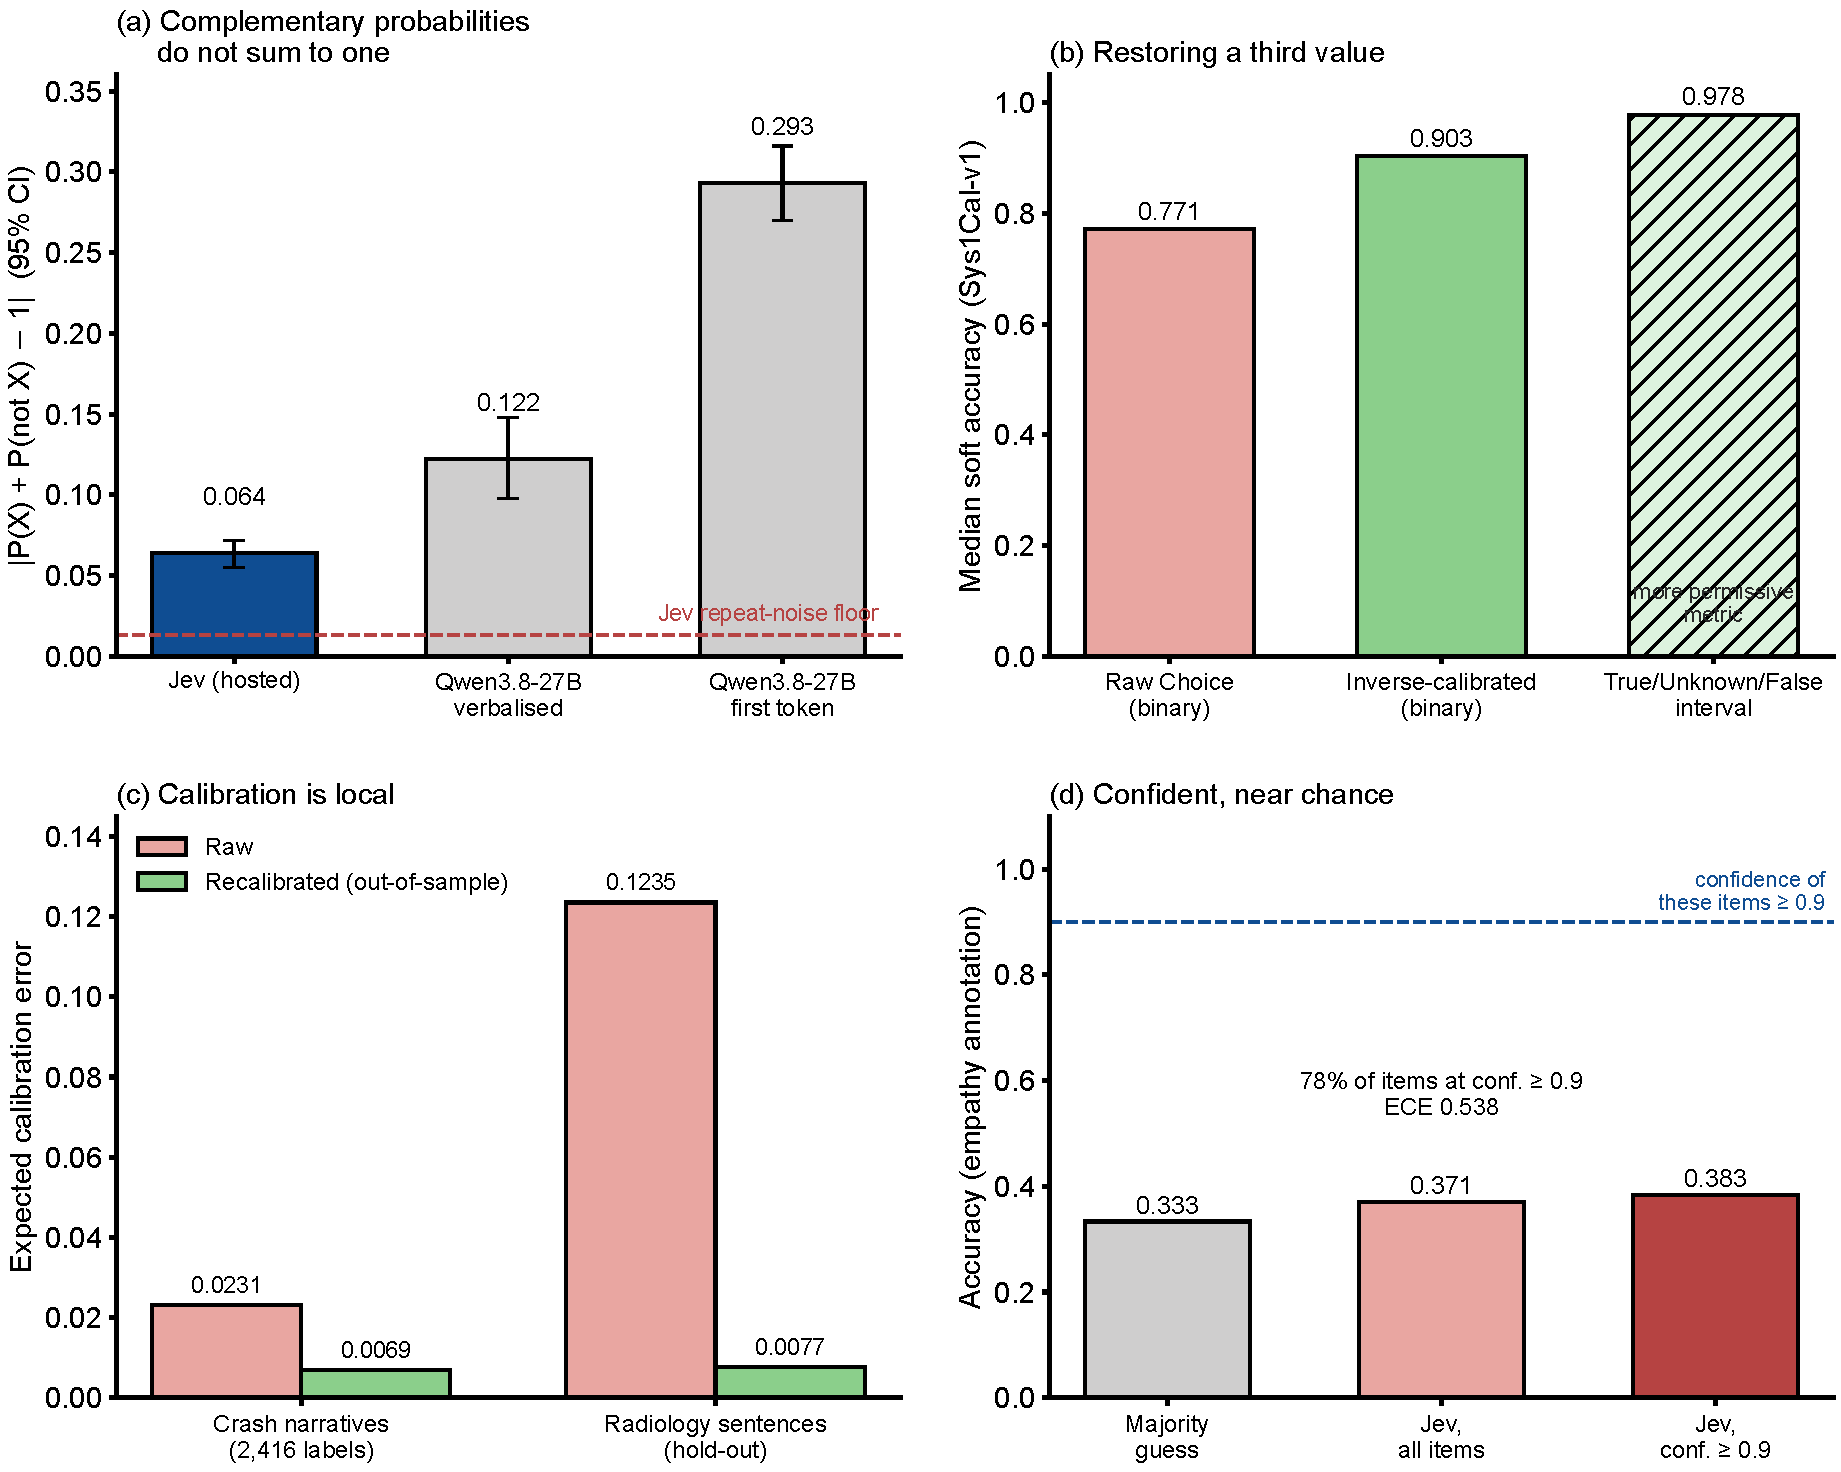
\includegraphics[width=0.9\linewidth]{figures/fig_honesty.pdf}
\caption{G4：诚实性。
(a) 480 个否定对上 $P(X)+P(\neg X)$ 偏离 1 的平均绝对偏差，与 \jev{} 的重复噪声下限对照~\protect\cite{arx33209}。
(b) Sys1Cal-v1 上的中位软准确率：原始 Choice 答案、校正被压制的“unknown”概率质量后（该研究的一个假设），以及采用更宽松的真/未知/假区间指标时（阴影）~\protect\cite{arx35342}。
(c) 基于本地标签重新校准前后的 ECE，采用折外方式~\protect\cite{arx24052}或留出集~\protect\cite{arx27607}。
(d) 共情标注（三个平衡类别）：\jev{} 在全部条目上及在其以置信度 $\geq 0.9$ 作答的条目上的准确率，与多数类基率对照~\protect\cite{arx24574}。}
\label{fig:honesty}
\end{figure}

% ---------------------------------------------------------------------------
\subsection{G5——仅为一个数值的决策能否被审计和解释？}
\label{sec:g5}

\begin{answerbox}
可以被记录和分解，但无法被解释。
类型化决策不返回理由，由多个问题或接口组合而成的决策未必一致；将中间事实作为独立步骤写入状态，可使链路可检查，且当这些事实正确时，可提高准确性，但在两项较晚的研究中，分解并未提高准确性（\cref{sec:update}）。
编码：S~2，Q~3，N~3。
\end{answerbox}

\paragraph{有记录而无理由。}
类型化模型只返回一个概率，别无其他，因此其输出中没有任何内容能表明是输入的哪一部分产生了判定~\cite{willison2026jev}。
一篇 Zenodo 评论认为，去除推理轨迹在结构上使责任归属更加困难~\cite{zen22847531}\zmark{}；另一篇认为，类型化推断可能将治理承诺转移到其开发者编写的模式、选项集、评分细则和阈值之中~\cite{zen22866847}\zmark{}。
当求解器在修改其逻辑谜题答案时被展示 \jev{} 的概率，其表现并不优于单纯再看一遍~\cite{zen22849329}\zmark{}。

\paragraph{可组合与不可组合的链路。}
在十个科学工作流中，\jev{} 正确完成了全部中间语义选择，而对照模型的七次错误选择（全部出现在同一问题上）改变了下游计数却未改变最终标签：仅凭最终标签准确率无法发现这些错误~\cite{arx24965}。
通过两种接口提问时，同一决策在 32.8\% 的案例中导致不同动作~\cite{arx37470}；由细粒度答案重构的类别概率与直接询问所得概率的平均总变差为 0.22--0.35~\cite{arx33971}；当条件发生变化时，逐步校准审计可能遗漏链路层面的错误~\cite{zen23064668}\zmark{}。
分解可以有所帮助：当 \jev{} 对对手动作的预测被写入状态时，其在误导性博弈中的决策正确率从 33\% 升至 94\%，但在给定一个错误的书面前提时，它在 26 次调用中有 24 次遵循该前提，这使书面事实本身成为审计点~\cite{arx01834}。

\paragraph{与已有工作的关系。}
决策后生成的解释未必反映产生该决策的因素~\cite{doshivelez2017towards}，而文档标准~\cite{mitchell2019model,gebru2021datasheets}描述的是模型和数据，而非单个决策；类型化保障机制需要一份决策记录，以及一份独立来源的理由陈述。

% ---------------------------------------------------------------------------
\subsection{G6——“有把握则执行，无把握则升级”是否可行？}
\label{sec:g6}

\begin{answerbox}
取决于升级的去向以及阈值的设定方式。
在若干研究中，将不确定案例升级至更强的推理模型，或仅接受经独立构建的规则确认的判定，节省了四分之一至一半以上的成本，且准确性无损失，但一项较晚的研究使这一发现有争议（\cref{sec:update}）；升级至同类模型则保留了高置信错误；在设定了预先固定阈值的研究中，多数研究的阈值在新数据上未能达到其错误目标，但在若干研究（包括一项预注册研究）中，\jev{} 的阈值达到了目标（\cref{tab:keyfindings}）。
编码：S~1，Q~23，N~4。
\end{answerbox}

\paragraph{有效的升级。}
\emph{JEV-as-a-Judge}~\cite{arx26550} 发现，在判定可直接从文本中读出的情形下，\jev{} 与 GPT-6 相差不超过三个百分点，费用仅为后者的 0.36\%，而在判定须经推导的情形下则明显落后。采用预先冻结的阈值，级联在 1{,}610 个留出配对上（83\% 来自 RewardBench；在 JudgeBench 上低 0.74 个百分点）以 GPT-6 费用的 41.4\% 超过 GPT-6 0.93 个百分点（CI 0.24--1.66），在针对两个新工作负载的前瞻性实时测试中，以各自 100 个本地标签设定阈值，它以 75.5\% 的费用与 GPT-6 持平（\cref{fig:escalation}a）。
在一项基于模拟网络数据、采用封存测试轮次的预注册研究中，仅当一个独立构建的规则树同意时才接受 \jev{} 的良性判定，使前沿 LLM 审核者得以跳过 34.5--38\% 的案例而 macro-F1 无损失，迁移至另外两个网络时亦然，但伪装攻击仍能通过（\cref{sec:g2}）~\cite{arx02048}。
一个预注册的标注级联以四分之一至一半的成本达到了仅用 LLM 的质量~\cite{arx24574}；一个采用不确定区间升级的语义数据库将平均 F1 从 63--66\% 提高到 96--98\%~\cite{arx02046}。

\paragraph{同类之间的升级。}
在一项评分细则打分研究中，\jev{} 的准确率与三个低成本生成式评估器之间，在 27 组配对比较中至多 8 组存在显著差异，而成本仅为后者的 $1/16$ 至 $1/325$~\cite{arx29769}。在七个有序评分面板上各取 \jev{} 置信度最高的 12 个错误（共 84 个条目），三个低成本生成式评估器在 252 次判定中有 242 次（96.0\%）给出了与 \jev{} 相同的错误答案，而若错误相互独立，预期比例为 50.3\%；由于这些条目是按 \jev{} 置信度最高的错误选出的，我们将此视为错误相关性的上界，尽管这正是对升级而言关键的条目集合~\cite{arx29769}（\cref{fig:escalation}b）。
重放已记录的判定时，最佳级联相对最佳单一评估器的平均增益至多为 1.5 个百分点，且在九个面板中的六个上低于后者（\cref{fig:escalation}c）。
在智能体安全筛查中，生成式评估器至多捕获了 \jev{} 130 次高置信漏检中的 5 次~\cite{arx33401}。
在另一项研究中，将 \jev{} 的不确定区间升级至低成本 LLM 从未带来显著帮助；只有成本为其 42--97 倍的前沿模型有所帮助，且仅在 30 个级联中的 2 个上，因此在低成本层级内，作者建议将该区间交由人工处理~\cite{zen22885291}\zmark{}。

\paragraph{阈值与门控。}
在 1\% 漏检限制下，对称的放行/阻断/审查策略在提示注入上对 \jev{} 未实现任何自动化，而独立阈值使 47.03\% 的交互风险案例实现自动化，且几乎全部通过额外的\emph{阻断}实现~\cite{arx33401}。
在一项预注册的标注研究中，预先固定的 0.9 置信度阈值本应带来至少 0.85 的准确率；实际中位准确率为 0.815，且在 14 项任务中有 8 项未达到~\cite{arx24574}。
在基于留出数据选定阈值的情况下，在一个匹配基准中，除一个模型外，每个模型实际风险的单侧上界均超过 5\% 的目标，而 \jev{} 的实际风险在一个数据集上达到目标（0.049），在另一个上未达到（0.058）；且为范围内请求设定的阈值使 \jev{} 接受了 31.0\% 的不在范围内的请求（设有显式“不在范围内”选项时为 19.5\%）~\cite{arx00346}。
基于置信度的暂缓判定在同分布条件下对一个由作者构建的医学类型化模型有效，其风险--覆盖率曲线下面积在四个任务族中的三个上低于匹配的生成式基线~\cite{arx00381}，且 \jev{} 自身的风险--覆盖率曲线在六项公开二分类任务上均为单调~\cite{zen22885291}\zmark{}；但在医学基准上，\jev{} 的选择性预测在三个中的两个上差于一个前沿模型~\cite{arx34024}。
0.8 的置信度门控放过了 12.6\% 由攻击引起的翻转，而一条插入的观点将 38.0\% 的高置信答案压至该门控以下~\cite{arx31142}。
一个基于 Laya 置信度构建的共形门控在名义水平 0.05 下返回的风险为 0.585~\cite{zen23041163}\zmark{}，一项预注册再现研究中冻结的 Laya 门控未达到其错误目标（0.140 对 0.10）~\cite{arx33843}。
在网络控制中，一个经微调的开源模型预先设定的门控未能迁移至变化后的问题：它在其中至多 0.801 的问题上错误执行，并在 7 个变化模板中的 6 个上超过 0.05 的目标；而 \jev{} 的门控（它会读取问题）在 7 个中的 6 个上保持在目标之内，在第七个上为 0.143，仍处于该研究的偏移界限之内；且一个共形标签下限意味着，要在 5\% 错误水平上认证对某一新问题类型的执行，至少需要该类型的 19 个标签~\cite{arx33689}。门控也可能有效：对 Kev-0.8B 而言，按覆盖率设定而非固定为 0.8 的阈值将所有被攻击从正确翻转为错误的答案送交审查，但强化既有错误的攻击可能通过~\cite{zen22959854,zen23038928}\zmark{}。

\paragraph{与已有工作的关系。}
级联与习得式暂缓判定已有定论~\cite{chen2023frugalgpt,madras2018predict,mozannar2020consistent}，模型间的相关错误亦然~\cite{goel2025great,verga2024replacing}；风险受控阈值~\cite{bates2021distribution,angelopoulos2024conformal}假定校准数据与部署数据之间可交换，而 G2 和 G4 的证据表明，在攻击或漂移下这一假定不会成立。
新的发现是，独立性必须被构建出来：一个以不同方式构建的规则有所帮助，同类模型则没有。

\begin{figure}[t]
\centering
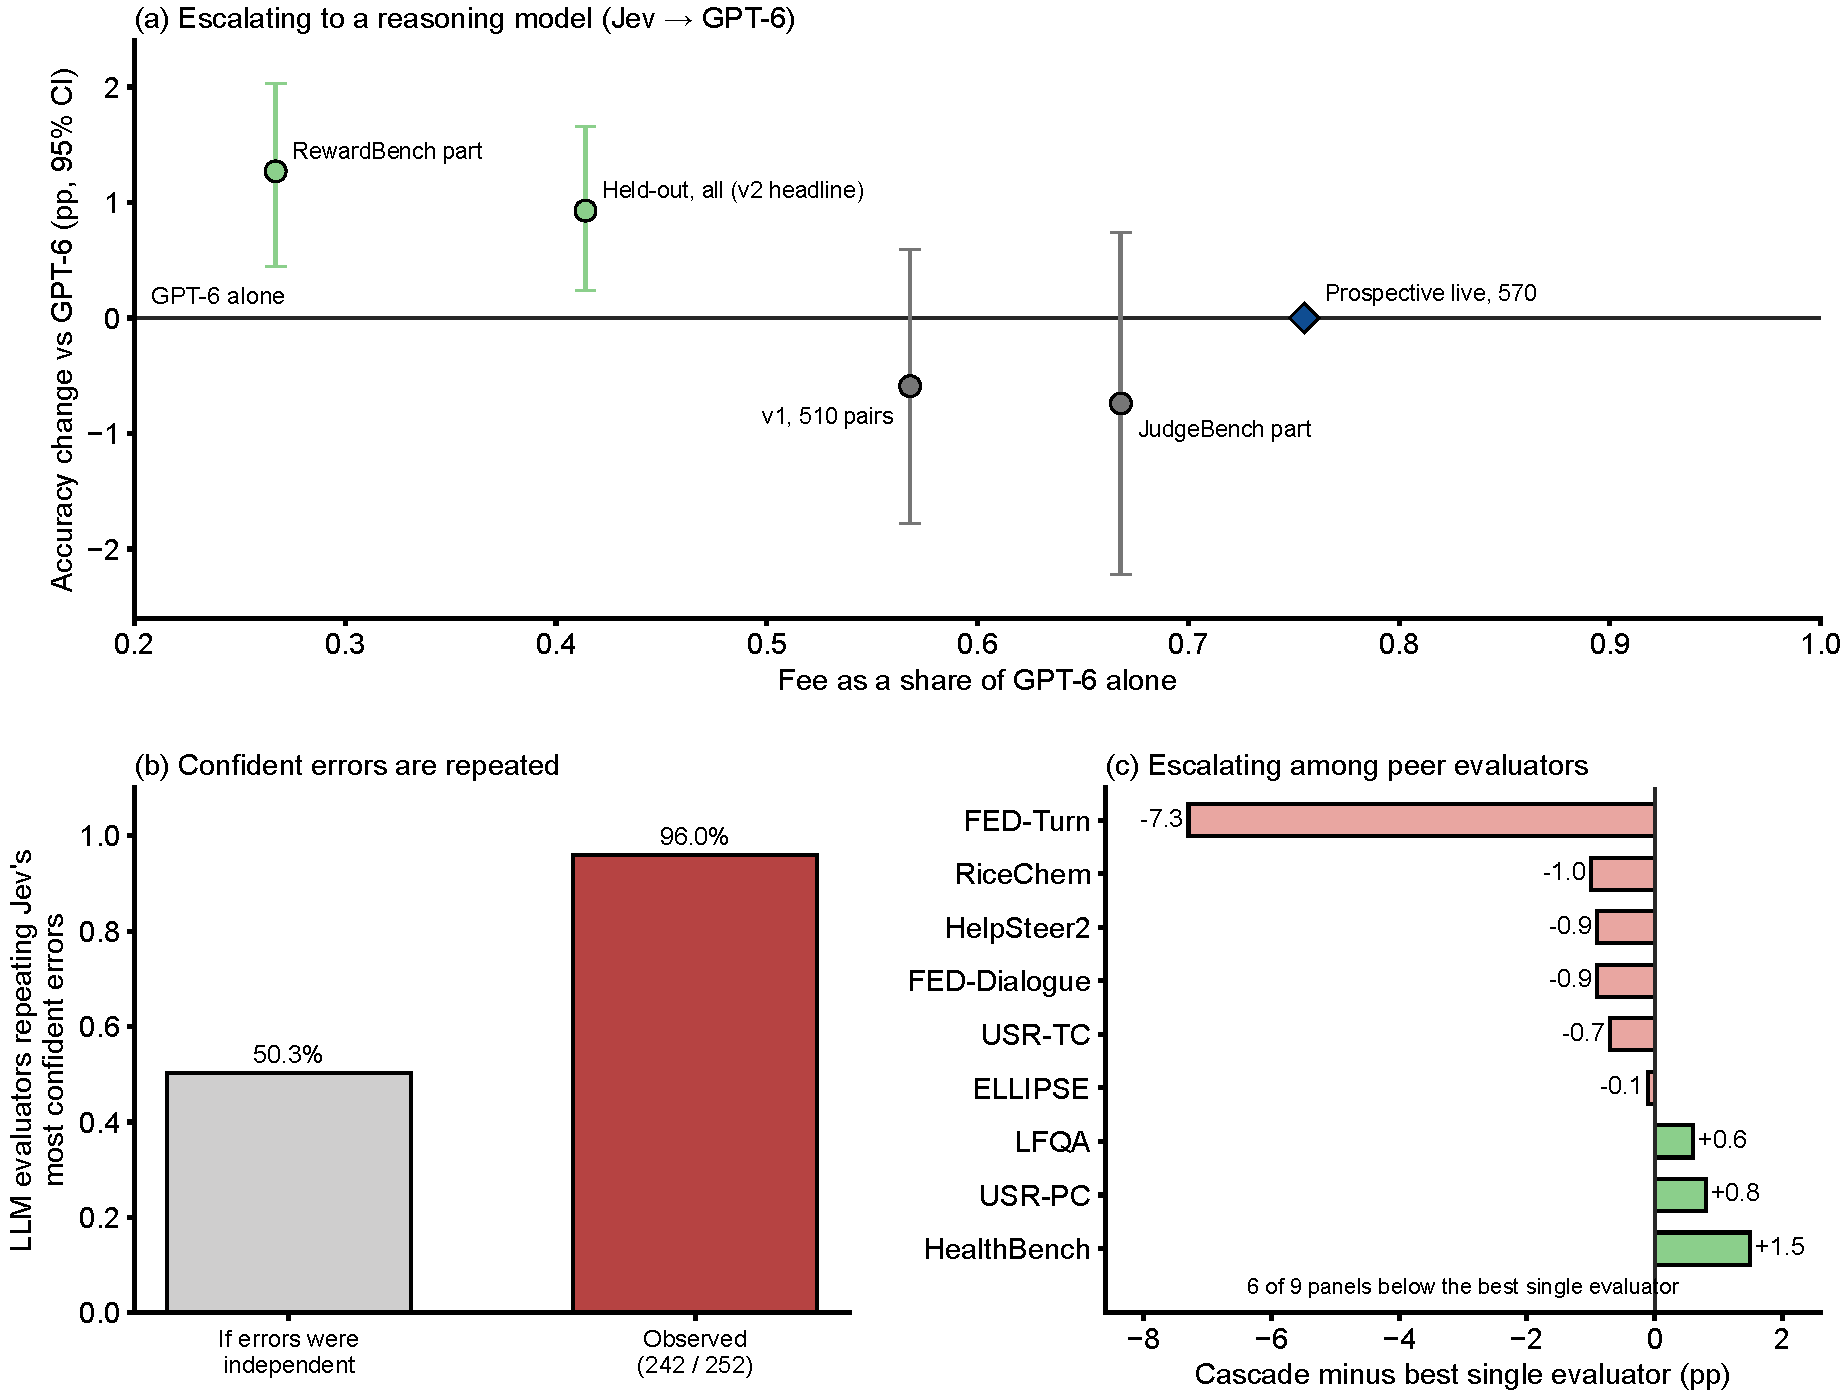
\includegraphics[width=0.9\linewidth]{figures/fig_escalation.pdf}
\caption{G6：升级。
(a) 从 \jev{} 到 GPT-6 的“有把握即接受”级联：准确率变化与费用占比~\protect\cite{arx26550}；灰色点的区间包含零，菱形为前瞻性实时测试。
(b) \jev{} 置信度最高的错误被低成本生成式评估器重复的比例，与错误相互独立时的预期比例对照~\protect\cite{arx29769}。
(c) 全部九个面板上交叉拟合级联减去最佳单一评估器的差值~\protect\cite{arx29769}。}
\label{fig:escalation}
\end{figure}

% ---------------------------------------------------------------------------
\subsection{G7——公共规模的判断与模拟}
\label{sec:g7}

\begin{answerbox}
类型化模型使人口规模的阅读与模拟变得廉价，部分研究展示了如何诚实地做到这一点：抽样审计，并将测得的与真实人群之间的差距带入每一项结论。
模拟公众偏向某一人群并低估分歧，且部署依赖于单一闭源厂商。
编码：S~5，Q~12，N~2。
\end{answerbox}

KITE~\cite{arx27535} 对每个唯一状态调用 \jev{} 一次，通过查表在一秒内模拟一百万个智能体，并将测得的人类--模型差异作为共享误差项传递至每一项结论；在 37 项未见研究上，该误差项在名义 80\% 和 90\% 水平下给出的回溯覆盖率分别为 0.93 和 0.96，高于名义水平，可能偏保守，但其预注册的主要终点未显示明显增益。
一项全州范围的研究用 \jev{} 阅读了约五十万份警方叙述，通过盲法人工裁定审计了一个按概率分层的样本，并报告了带区间的、经误分类校正的计数，同时发现在两轮脱敏后，记录胎儿伤害的叙述中有 43\%、裁定样本中有 37\% 仍残留个人标识信息~\cite{arx00213}。
在无人设时，\jev{} 回答价值观问题的方式与其美国人设相似，并在标注者意见分歧之处保持高置信（\cref{sec:g3,sec:g4}），因此模拟公众偏向某一人群并低估分歧~\cite{arx36399,zen23032384}\zmark{}。
匹配基准显示，托管 \jev{} 每千次决策成本不足一美分，中位延迟为 138\,ms~\cite{arx00346}；其权重未公开，也不提供自托管，这促使一项路由研究将其接口设计为与分类器无关，并配备自托管的后备方案~\cite{arx28919}。
一篇概念性论文认为，更廉价的评估可能增加而非减少评估总量和异常处理~\cite{arx01231}。
此处的诚实性条件即调查方法论和关注分歧的标注~\cite{davani2022dealing,plank2022problem}所要求的条件。

% ---------------------------------------------------------------------------
\subsection{跨要求综合}
\label{sec:across}

在 \nRows{} 个已编码的研究--要求配对中，\nS{} 个支持检测器用途，\nQ{} 个为有条件（Q），\nN{} 个为不支持（N）（\cref{fig:framework}）。
仅保留较强设计的研究时（\nStrongRows{} 个中 \nStrongS{}、\nStrongQ{} 和 \nStrongN{} 个），或剔除 Zenodo 记录时（Zenodo 记录被编码为 N 的比例高于 arXiv 论文：44 个配对中 19 个，对 107 个中 25 个；剔除后为 \nNoZenRows{} 个中 \nNoZenS{}、\nNoZenQ{} 和 \nNoZenN{} 个），各比例变化约六个百分点或更少。
七十六个配对在同一要求上将类型化模型与生成式评估器进行了比较：类型化模型在 23 个中更好，17 个中相近，28 个中不一，8 个中更差。
具体就失效而言，图景更为单薄且更不利：在有对照的 14 个 N 编码中，类型化模型在 6 个中更差，4 个中相近，3 个中不一，1 个中更好；而 48 个 N 编码中有 34 个完全没有对照。
因此，证据既未表明类型化模型总体上差于生成式评估器，也未表明其失效与后者共有；对多数失效而言，这一比较尚未进行。
有两种失效模式源于类型化接口本身：所报告的置信度可能因填充选项集而被抬高（G4），且决策不附带理由（G5）；第三种，即概率向量为攻击者提供指引，仅在一项研究中得到证明（G2）。

综合来看，这些编码仅在全文所用的限定意义上支持检测器用途：几乎每一项成功都依赖于某一附加条件，如本地拟合的阈值、第二道独立核查或人工审查；而 G2 和 G4 中的失效是检测器本身的失效，因为被操纵或沉默的检测器会漏掉违规。因此，\cref{sec:design} 的建议并非认为类型化检测器可靠，而是认为：在检测器角色中（每一项具有实质后果的动作都须经过另一道核查），其失效比在裁决者角色中（没有任何此类核查）更易于以较低代价加以控制。

\Cref{tab:keyfindings} 列出了被纳入\cref{sec:synthesis,sec:design}及摘要的发现，并给出各自的确定性：按\cref{sec:appraisal}的规则评定，纳入主窗口和更新检索中与该发现相关的全部已编码研究；为便于比较，同时列出 10 月 4 日给定的评级。没有任何发现达到中等确定性，有四项发现有争议。

\begin{table}[!htbp]
\centering
\footnotesize
\setlength{\tabcolsep}{3pt}
\caption{主要发现及证据确定性。\emph{范围}：托管 \jev{}、开源模型或两者（泛指类型化模型）；关于托管 \jev{} 或两者的发现仅依据托管模型证据评级，按系统组计数。\emph{编码}：支持研究的编码。\emph{来源}：先列主要支持研究，再列相反研究（计入的每项研究及其方向均列于 \nolinkurl{data/certainty_evidence.csv}）；“更新：”为更新检索研究；“开源：”为开源模型研究，起佐证作用（标为“开源，反向：”者则指向相反方向），但不计入评级。确定性的定义见\cref{sec:appraisal}；$^{c}$~在该范围内有争议；$^{j}$~依判断评级的描述性计数。\emph{10 月 4 日}：10 月 4 日给定的评级（所引研究，旧规则）；$^{a}$~按现行规则为极低（\cref{sec:certainty-detail}）。\emph{当前}：现行规则，纳入全部已编码的主窗口与更新研究（仅主窗口：\cref{tab:certchanges}）。由 \nolinkurl{scripts/rate_certainty.py} 根据 \nolinkurl{data/certainty_evidence.csv} 计算。}
\label{tab:keyfindings}
\begin{tabularx}{\linewidth}{@{}L>{\raggedright\arraybackslash}p{0.06\linewidth}>{\raggedright\arraybackslash}p{0.055\linewidth}>{\raggedright\arraybackslash}p{0.12\linewidth}>{\raggedright\arraybackslash}p{0.17\linewidth}>{\raggedright\arraybackslash}p{0.08\linewidth}>{\raggedright\arraybackslash}p{0.08\linewidth}@{}}
\toprule
发现 & 范围 & 编码 & 与生成式比较 & 来源 & 10 月 4 日 & 当前 \\
\midrule
零样本下对有害或未对齐内容排序良好，成本仅为一小部分；常不及最佳 LLM 准确 & 托管 & S/Q/N & 更好（低成本）；更差（最佳） & \cite{arx29429,jkf87_2026replication,zen22885291,arx33401,arx24574,arx27678} & 低 & 低 \\
固定阈值不可迁移；需本地拟合 & 两者 & Q & -- & \cite{arx29429,jkf87_2026replication,arx00346,arx01006,arx26550,arx24574,arx02046}；相反：\cite{arx33689}；更新：\cite{arx03387,arx02267,zen22935043} & 低 & 低$^{c}$ \\
错误集中于被总体指标掩盖的子类型 & 托管 & Q & 不一 & \cite{arx33401,alphaRAG,arx02046}；更新：\cite{arx07953,arx03324,arx08675,arx10321} & 极低 & 低 \\
插入的观点、经优化的上下文和词汇诱饵可操纵决策 & 两者 & N & 相近 & \cite{arx31142,arx01834,arx01006,arx30243,arx02048}；开源：\cite{zen22959854,zen23038928} & 低 & 低 \\
指令注入很少选中攻击者的目标（原始 1.8\%，自适应 3.5\%） & 托管 & S & -- & \cite{arx28613}；相反：\cite{arx31142,checkpoint2026jev}；更新，相反：\cite{arx04985} & 极低 & 极低$^{c}$ \\
选项名称可能压过定义；中性标识符可消除其大部分 & 两者 & N & -- & \cite{arx26758,arx00346}；更新：\cite{arx07953}；开源：\cite{arx02586} & 低 & 低 \\
默认偏向某一种文化的价值观 & 托管 & N & -- & \cite{arx36399} & 极低 & 极低 \\
在熟悉的封闭选择任务上校准良好，与前沿模型相比结果不一；校准是局部的 & 托管 & S/Q & 更好或不一 & \cite{arx37647,arx01006,arx24052,arx27607,arx24574,arx34024,zen22885291} & 低 & 低 \\
显式“不知道”在正确时很少被选中；“以上皆非”的选择不一致 & 托管 & Q/N & 相近或更差（前沿）；更差（推理） & \cite{arx34024,arx39496,arx01006}；更新：\cite{arx03387,arx06425} & 低 & 低 \\
另设的充分性问题可检测信息缺失，但筛选答案的效果不如置信度 & 托管 & Q & -- & \cite{arx01006} & 极低 & 极低 \\
升级至更强的推理模型可在可读出的判断上节省成本且准确性无损失 & 两者 & Q & 相近 & \cite{arx26550,arx24574,arx02046}；开源：\cite{zen22922769}；更新，相反：\cite{arx02267}；开源，反向：\cite{arx07177,arx03324} & 低 & 低$^{c}$ \\
以与独立构建规则一致为接受条件，macro-F1 无损失，但被标记的伪装攻击更少 & 两者 & Q/N & 相近 & \cite{arx02048}；更新，开源：\cite{zen22904595} & 极低 & 极低 \\
同类评估器重复 \jev{} 置信度最高的错误（上界） & 托管 & N & 相近或不一 & \cite{arx29769,arx33401} & 低 & 低 \\
预先设定的阈值在新数据上未达到错误目标 & 两者 & Q/N & -- & \cite{arx33401,arx24574}；相反：\cite{arx33689}；开源：\cite{arx33843,zen23041163,arx07177}；更新：\cite{arx03387,arx02267}；更新，相反：\cite{zen22935043,zen23075657} & 中等$^{a}$ & 低$^{c}$ \\
类型化模型总体上并不差于生成式评估器；多数失效缺乏对照比较 & 两者 & -- & 76 个中 23 个更好、8 个更差 & \cref{app:evidence} & 低 & 低$^{j}$ \\
尚无研究测量 \pol{} 构念（三值、中文） & -- & -- & -- & -- & -- & -- \\
\bottomrule
\end{tabularx}
\end{table}

\FloatBarrier

% ---------------------------------------------------------------------------
\subsection{更新检索（2026 年 10 月 2--8 日）}
\label{sec:update}

更新检索（\cref{sec:search}）新增 \nUCoded{} 个已编码来源：\nUSetPostWindow{} 个于 10 月 2--8 日首次发布，\nUSetLateIndexed{} 篇为迟索引的 arXiv 论文，\nUSetReScreened{} 条为重新筛选的 Zenodo 记录。
其 \nURows{} 个研究--要求配对的编码为 S~\nUS{}、Q~\nUQ{}、N~\nUN{}（仅较强设计研究：\nUStrongRows{} 个中 \nUStrongS{}、\nUStrongQ{} 和 \nUStrongN{} 个）；这些配对未合并入上文的计数，\cref{tab:update} 将其与主窗口并列。
作为敏感性检验，我们将日期在主窗口之内的 18 条记录（36 个配对：S~5，Q~28，N~3）加入主计数；这不改变任何简要回答，最常见的编码仅在主窗口中 Q 与 N 几乎持平之处发生变化（G3：N~12 对 Q~10 变为 Q~14 对 N~13；G5：3--3 持平变为 Q~4 对 N~3）。
该检验仅涉及编码的方向；它不重新计算对照比较的比例，而\cref{tab:keyfindings} 中的确定性评级是在加入全部更新研究（包括这 18 项）后评定的。
更新集合中 N 编码的比例低于主窗口（配对的 12\% 对 30\%）：仅有一项新研究攻击了类型化模型（G2，即编码最为不支持的要求），且多数新配对的结果不一。
在其 14 个 N 编码中，9 个有生成式对照，其中类型化模型在 6 个中更差，这 6 个中有 4 个仅涉及开源模型；两个集合合计，62 个 N 编码中仍有 39 个缺乏对照。

没有任何简要回答被推翻。
新证据限定了一项表述，即 G5 中关于分解链路的表述，该简要回答已相应修订；其他简要回答不变，新证据大多对其予以确认。
\cref{sec:appraisal} 的确定性规则在评审期间（这些研究完成编码之后）进行了修订，每项发现均依据全部已编码的主窗口和更新研究按该规则重新评级；这构成一项方案偏离，因为更新方案原已冻结主窗口的评级。
与仅依据主窗口研究相比，更新研究改变了一项评级：两项关于托管 \jev{} 的较强设计研究将“预先设定的阈值在新数据上未达到错误目标”这一发现从极低提升至低，但仍有争议~\cite{arx03387,arx02267}，另有两项研究的阈值达到了目标，增加了相反证据~\cite{zen22935043,zen23075657}\zmark{}。更新研究还使“升级至更强的推理模型”这一发现有争议，因为一项 \jev{} 预筛仅使一个安全审核者的成本降低 4.3\%~\cite{arx02267}；并为注入发现（主窗口中已有争议）增加了一项相反研究。
各项发现的推导过程及相对 10 月 4 日的变化见\cref{sec:certainty-detail}。
下文按要求逐项给出与 \pol{} 最直接相关的研究。

\begin{table}[!htbp]
\centering
\footnotesize
\caption{主窗口与更新检索中按要求划分的编码（S/Q/N）。\emph{更新}：全部更新配对；\emph{窗口内}：来自 \nUSetLateIndexed{} 篇迟索引 arXiv 论文和 \nUSetReScreened{} 条重新筛选 Zenodo 记录、日期在主窗口之内的配对；\emph{主窗口 + 窗口内}为敏感性检验。最后一列：有生成式（生成）对照的更新配对中，类型化模型更好、相近、不一或更差的数量，以及无对照的配对数。数据：\nolinkurl{data/evidence_coding_update_2026-10-08.csv}。}
\label{tab:update}
\begin{tabular}{@{}lccccc@{}}
\toprule
要求 & 主窗口 & 更新 & 窗口内 & 主窗口 + 窗口内 & 更新与生成式比较；无 \\
\midrule
G1 & 2/20/5 & 2/17/3 & 1/9/0 & 3/29/5 & 1/4/7/3；7 \\
G2 & 1/0/9 & 0/0/1 & 0/0/0 & 1/0/9 & --；1 \\
G3 & 2/10/12 & 5/15/3 & 1/4/1 & 3/14/13 & 3/2/3/0；15 \\
G4 & 3/29/13 & 3/26/3 & 2/6/1 & 5/35/14 & 6/0/7/3；16 \\
G5 & 2/3/3 & 0/6/0 & 0/1/0 & 2/4/3 & 1/1/2/0；2 \\
G6 & 1/23/4 & 1/19/3 & 1/7/1 & 2/30/5 & 3/3/2/0；15 \\
G7 & 5/12/2 & 1/9/1 & 0/1/0 & 5/13/2 & 1/0/6/1；3 \\
\midrule
全部 & \nS{}/\nQ{}/\nN{} & \nUS{}/\nUQ{}/\nUN{} & 5/28/3 & 21/125/51 & 15/10/27/7；59 \\
较强设计 & \nStrongS{}/\nStrongQ{}/\nStrongN{} & \nUStrongS{}/\nUStrongQ{}/\nUStrongN{} & -- & -- & -- \\
\bottomrule
\end{tabular}
\end{table}

\paragraph{G1：得到确认。}
三项新研究检验了仇恨言论与内容审核，即安全阀的核心。
在未经任务训练的情况下，\jev{} 在四个英文数据集上的二分类仇恨言论 macro-F1 分别为 0.826、0.691、0.738 和 0.960，而 GPT-6 Sol 为 0.897、0.682、0.776 和 0.976；商用 LLM 仅在一个数据集上显著领先于每一个决策模型；所有模型（类型化与生成式）均难以区分仇恨言论与仅具冒犯性的语言（三分类：\jev{} 0.532，Sol 0.604，一个监督式 TF-IDF 分类器 0.639）~\cite{arx03324}。
这比“常低于最佳评估器”所暗示的更接近最佳 LLM，但仍在简要回答所述方向之内。
在在线内容审核中，\jev{} 在两个英文数据集上的 F1 与 Detoxify 持平或更高（但其在其中一个数据集上的准确率较低，74.4\% 对 81.0\%），在一个 Bluesky 基准上的 AUROC 为 0.89--0.90；但其在 Facebook 仇恨言论政策选择上的精确匹配准确率在无检索先例时为 29.4\%（有先例时为 51.6\%），在一个社区规则测试集上的得分低于始终回答“no rule broken”（未违反任何规则）（48.4\% 对 50.0\%）~\cite{arx07953}。
在 ToxicChat 上，基于 1{,}000 个开发标签选定的阈值，在一个由先前已观测条目构成、带混合标签的测试集上，以 3.24\% 的误报率取得 90.52\% 的召回率，处于该研究 5\% 的容差之内，而三种固定编码器条件的召回率为 35.6--58.9\%；在一项事后细分中，仅就人工标注的负例而言，误报率为 5.39\%~\cite{zen23075657}\zmark{}。
作为提示注入、越狱、有害内容和 AI 生成文本的零样本检测器，托管 \jev{} 在八个基准上的 AUROC 为 0.95--1.0，但其准确率（在六个安全基准上为 87--99\%）是在基于留出样例拟合的阈值下测得的；在 AI 生成文本上，准确率仅在采用此类阈值时才从默认阈值下的 78\% 升至 89\%~\cite{arx04985}；在一个智能体测试框架中，它对注入的筛查效果良好（AUROC 0.98），却放过了 25.5\% 的有害请求，且无法用作个人数据门控（误报率 63--66\%）~\cite{arx02267}。
在 AgentHarm 的有害性判断上，在单次运行中它与九种生成式配置中的最佳者持平（84.54\% 对至多 85.57\%）~\cite{arx03935}。
总体指标再次掩盖了子类型失效：在已编码字段同时记录了该因素的情形下，人工编码者确认了 \jev{} 交通事故叙述标记的 96--100\%，但对未系安全带的乘员为 15\%~\cite{arx10321}；该研究是对~\cite{arx24052}的扩展，出自同一作者并使用复用数据，因而与之并不独立。
两个开源类型化模型在相同基准上的得分低于生成式对照~\cite{arx06744,arx07177}；在工业故障检测中，托管 \jev{} 标记了 57--94\% 的无故障窗口，并且在九项偏移测试下，其表现并不优于标记每一个窗口~\cite{arx09937}。

\paragraph{情绪与中文文本（T1）。}
在八个情感基准上进行零样本测试，\jev{} 的平均 macro-F1 为 62.93\%，高于十种生成式配置中的五种，低于最佳者（67.28\%），成本比最佳者低 96\%；在中文情绪分类（CMMA）上，所有系统表现均弱（\jev{} 21.06，生成式模型 19.82--23.31）~\cite{arx08829}。
这项单次运行研究分类的是文本所表达的情绪，而非人的状态，因此它涉及的是 T1 会保留的边界一侧（\cref{sec:synthesis}）：如今为每条消息给出情绪分数已很廉价，而在中文文本上这些分数并不准确。
没有新研究在中文上操纵语言；一项基于中文请求构建的工程基准在 G4 下讨论~\cite{arx09896}。

\paragraph{G2：得到确认。}
一项新研究攻击了托管 \jev{}：一种针对 \jev{} 的注入和一个通用后缀在三项任务上达到 97--100\% 的攻击成功率，且投毒 5--10\% 的训练数据即在一个开源模型中植入了后门~\cite{arx04985}。
这一攻击的成功率远高于主窗口中那项支持研究中的攻击（1.8\% 的目标选中率）~\cite{arx28613}，后者使用的是不同的攻击和基准；该发现此前已因针对托管 \jev{} 的其他攻击而有争议~\cite{arx31142,checkpoint2026jev}，其确定性仍为极低。

\paragraph{G3：得到确认。}
为每个仇恨言论数据集提供其自身的定义，改变了决策模型 2.8--27.9\% 的预测，显著提升与显著下降同样频繁（28 次比较中各 8 次）；\jev{} 最不敏感，而一个经政策训练的生成式模型在四个数据集中的三个上一致性也有所下降~\cite{arx03324}。
将不透明的政策标识符替换为可读的仇恨言论政策名称，使 \jev{} 的二分类准确率下降 5.06 个百分点（CI 3.91--6.21）~\cite{arx07953}；在三个开源 Laya 检查点中，与其定义相矛盾的标签使准确率降至 0.14，低于无信息对照~\cite{arx02586}。
然而，中性标识符并非没有代价：在匹配对照中，它们使一个开源生成式读出对缺失答案的检测下降 20--31 个百分点~\cite{arx03387}。
选项顺序对托管 \jev{} 的影响远小于对开源类型化模型的影响（决策变化率 1.8\%，Laya 为 30.3\%~\cite{arx02267}；顺序敏感性 0.039，Laya 各变体为 0.37--0.59~\cite{arx02293}），且 \jev{} 的顺序一致性高于 Qwen3-32B~\cite{arx09188}，与“稳健性因模型而异”一致；但改写定义或以不同方式呈现相同证据仍会改变其答案~\cite{arx09937,arx08675}，且顺序翻转集中于其不确定之处~\cite{arx06625}。
一个基于挪威和奥地利登记册文本训练的开源模型，在奥地利测试集中 94.6\% 的规则类型上与参考一致，而在一个未见过的丹麦登记册上为 62.4\%~\cite{zen23225893}\zmark{}。

\paragraph{G4：得到确认。}
与前沿模型的比较结果仍然不一。
在一个包含 10{,}938 个问题的双语基准上，\jev{} 的 ECE 低于所有生成式配置（0.053 对 0.078--0.253），但它将 89\% 的概率质量置于众数上，而真实比例为 36\%~\cite{arx03935}；在八项人工标注的阅读任务上，它的校准优于一个前沿模型的词元概率，但在成对任务上，一个 27B 开源模型校准更好~\cite{arx06625}；在中文工程问题上，其 ECE 为 0.027，而三个旗舰 LLM 的自述概率为 0.031--0.061，尽管它在 5{,}000 条记录中有 678 条失败~\cite{arx09896}；在其自身生成的博弈状态中，它差于常数预测器（Brier 0.283 对 0.250），而一个通过选项概率读出的小型生成式模型胜过该常数预测器~\cite{zen23221456}\zmark{}。
在冒犯性语言和仇恨言论任务上，无检索先例时其概率校准不佳（OLID 上 ECE 14.9\%，HateXplain 上 33.2\%；有先例时为 9.7\% 和 20.2\%）~\cite{arx07953}。
在弃权方面，设有显式 NONE 选项时，\jev{} 在正确答案被人为移除的条目中拒绝了 63.7\%，错误拒绝率为 3.3\%（一个开源生成式读出：45.0\%），在第二项任务上为 82.4\%，但随着候选项增加，检测率下降~\cite{arx03387}；未针对该任务训练的托管 \jev{} 对 382 个不可回答条目中的 62.8\% 给出了确定答案，而作者的循环（looped）模型为 17.5\%~\cite{arx07730}；在一个开源 \jev{} 式读出中，显式 ABSTAIN 选项拒绝了 30 个无有效答案案例中的 28 个，但在 30 个有效案例中仅 17 个选择正确~\cite{arx07327}。
在提供拒绝或升级选项时，托管 \jev{} 在 48 份无有效候选的合同中有 45 份请求新候选，但在 120 个无可行路径的转发实例中仅升级了 4 个~\cite{arx06425}。
这些结果与简要回答相符：显式的“不足”选项仅部分有效，且“以上皆非”（none）的选择不一致——在关于托管 \jev{} 的各项研究中，对无答案条目的选择比例为 3--94\%~\cite{arx39496,arx03387,arx06425}。

\paragraph{G5：一项表述受到限定。}
两项研究将一个判断分解为若干标准问题并以固定规则组合：在仇恨言论上，这在 30 次比较中有 6 次提高、11 次降低了 macro-F1，且 \jev{} 的唯一一次提升可由调优后的阈值同样达到~\cite{arx03324}；在八个情感基准上，它使 \jev{} 的平均值从 62.93\% 降至 57.31\%，而将这些判断附加到状态中也未更准确（61.61\%）~\cite{arx08829}。
在另外两项研究中，仅暴露与当前步骤相关的字段，或将核查移入一个单独的门控，提高了正确决策数（120 个中从 90 增至 113；120 个中从 29 增至 84）~\cite{arx07327,arx06425}。
因此，分解可使链路可检查，但仅在部分情境下提高准确性，G5 的简要回答现已如此表述。
一个概念验证记录并重构了两个实时决策，但仅在其作者构建的确定性外壳之内，且输出不附带理由~\cite{zen23189584}\zmark{}，这确认了“可以被记录，但无法被解释”。

\paragraph{G6：得到确认，但一致性较低。}
预先固定的阈值在新数据上常常未达到其目标，但并非总是如此：在一项任务上校准的拒绝阈值，在 12 次迁移中有 6 次超过了 5\% 的错误拒绝目标~\cite{arx03387}；分裂共形预测达到了其边际目标，尽管在该方法下 \jev{} 的单标签答案在名义 5\% 水平下有 5.93\% 是错误的~\cite{zen22935043}\zmark{}；基于训练登记册拟合的弃权阈值在奥地利测试集上守住了预注册的 2\% 目标（1.3\%），但在一个未见过的登记册上产生了 14.3\% 的风险，而目标为 5\%~\cite{zen23225893}\zmark{}。
认证也可能拒绝给出：在同一研究中，一种界限为近似界限而非精确有限样本界限的程序，在 2{,}000 次划分中的任何一次上都无法为 \jev{} 在 AG News 上认证 5\% 的自动层级（在 SST-2 上为 2{,}000 次中的 191 次）；一种探索性的替代阈值规则在 2{,}000 次 SST-2 划分中认证了 1{,}776 次，但在 AG News 上仅 4 次~\cite{zen22935043}\zmark{}。
在内容审核中，仅接受置信度 $\geq 0.8$ 的 \jev{} 决策覆盖了一个 Bluesky 基准的 71.9\%，准确率为 94.3\%，但在仇恨言论政策选择上，被接受决策的准确率仅为 75.8\%，在社区规则上为 67.6\%~\cite{arx07953}。
升级至更强的推理模型在部分研究中有所帮助：以推理模型 30\% 的调用次数达到与之相当的水平~\cite{arx09683}；在一项探索性分析中，由前沿模型（GPT-6 Sol）复核 Laya 最不确定的五分之一条目提高了仇恨言论 macro-F1，但在三个数据集中的两个上未达到该前沿模型自身的水平，而转交一个更廉价的模型（GPT-5.6 Luna）则在一个数据集上使其下降~\cite{arx03324}；但在另一些研究中并无帮助：一个从接近随机水平的开源类型化评估器出发的预注册级联几乎将每个条目都升级~\cite{arx07177}，而在计入其自身词元后，\jev{} 预筛仅使一个 LLM 安全审核者的成本降低 4.3\%~\cite{arx02267}。
将 \jev{} 最不确定的重排序标签升级至 Qwen3-32B 从未带来帮助~\cite{arx09188}；在该任务上，Qwen3-32B 的准确性与 \jev{} 大致相当（与人工评分者的一致率 87.2\% 对 86.2\%，但重排序器 NDCG@10 略低，0.630 对 0.637），因此计为同类模型（\cref{sec:appraisal}），该结果正是简要回答对同类模型所预期的。
在由独立构建的核查掌握决定权之处，依据类型化决策采取行动是安全的~\cite{arx07327}；一个预先固定且带有基于规则后备方案的门控在新数据上保持有效~\cite{zen23088660}\zmark{}。
简要回答仍然成立，但关于升级可节省成本且准确性无损失的证据不如主窗口中一致：其确定性仍为低，且该发现现已有争议（\cref{tab:keyfindings}）。

\paragraph{G7：得到确认，并新增一项关于隐私的不支持证据。}
在 HateCheck 上，\jev{} 每 1{,}000 条文本的成本为 0.033 美元，中位延迟 336\,ms，而 GPT-6 Sol 为 1.177 美元和 1{,}426\,ms，\jev{} 的 macro-F1 比后者低 1.6 个百分点~\cite{arx03324}；但在七项政治学任务中的六项上，按批量价格计算，它并不比前沿模型便宜~\cite{arx06625}。
对 229{,}510 份交通事故叙述的两层概率抽样给出了经盲法人工层确认的全州计数，但这仅在逐因素的人工重新校准之后才实现~\cite{arx10321}，即简要回答所描述的设计。
作为群体投票分布的替代，\jev{} 的 Choice 概率在人们以 55 比 45 分歧的安全条目上报告了 0.88，表现差于均匀猜测~\cite{zen23179064}\zmark{}，这确认了它会低估分歧。
新的是关于隐私与双重用途的证据：用户输入中的条件指令使托管 \jev{} 仅凭其标签即在每个受测案例中泄露了隐藏的性别、年龄组、心脏病和族裔属性；\jev{} 被用作判定接口（oracle），提高了有害计划被评判的有害性；其 200 个标签将一个替身模型的一致率从 49\% 训练至 92\%~\cite{arx04985}。
这将不向不受信任的调用方提供概率的理由（\cref{sec:design}）扩展至放入检测器输入中的字段，以及不受信任的调用方可查询的任务。
